% Created 2018-12-05 Wed 21:42
% Intended LaTeX compiler: pdflatex
\documentclass[11pt]{article}
\usepackage[utf8]{inputenc}
\usepackage[T1]{fontenc}
\usepackage{graphicx}
\usepackage{grffile}
\usepackage{longtable}
\usepackage{wrapfig}
\usepackage{rotating}
\usepackage[normalem]{ulem}
\usepackage{amsmath}
\usepackage{textcomp}
\usepackage{amssymb}
\usepackage{capt-of}
\usepackage{hyperref}
\author{rkabrick}
\date{\today}
\title{}
\hypersetup{
 pdfauthor={rkabrick},
 pdftitle={},
 pdfkeywords={},
 pdfsubject={},
 pdfcreator={Emacs 26.1 (Org mode 9.1.9)},
 pdflang={English}}
\begin{document}

\tableofcontents

\%++++++++++++++++++++++++++++++++++++++++
\% Don't modify this section unless you know what you're doing!
\documentclass[letterpaper,12pt]{article}
\usepackage{tabularx} \% extra features for tabular environment
\usepackage{amsmath}  \% improve math presentation
\usepackage{graphicx} \% takes care of graphic including machinery
\usepackage[margin=1in,letterpaper]{geometry} \% decreases margins
\usepackage{cite} \% takes care of citations
\usepackage[final]{hyperref} \% adds hyper links inside the generated pdf file
\hypersetup\{
	colorlinks=true,       \% false: boxed links; true: colored links
	linkcolor=blue,        \% color of internal links
	citecolor=blue,        \% color of links to bibliography
	filecolor=magenta,     \% color of file links
	urlcolor=blue
\}
\%++++++++++++++++++++++++++++++++++++++++


\begin{document}

\title{CPEG466 Report}
\author{Ryan Kabrick}
\date{December 8th, 2018}
\maketitle

\begin{abstract}
This semester I have completed several different tasks for CAPSL. These tasks range from sorting and cleaning out Professor Gao's library of books to successfully implementing programs like Ansible and MPI on the full 24 node cluster. While there is still countless projects to be completed, this is a summary of my work in the past few months.
\end{abstract}


\section{Cluster}
I have spent a majority of my time working on the cluster of Parallella boards. With both Jose and Diego's help, I...
\begin{itemize}
\item Created a master image for the SD cards which included the necessary programs for the cluster including
  \begin{enumerate}
  \item \textbf{Ansible}: A way to automate parts of the cluster along with sending a single command to all of the nodes at once
  \item \textbf{MPI}: A program that allows for the distribution of computation across many different nodes
  \item \textbf{I'll fill this in later}
  \end{enumerate}
\item Updated/Rewrote the documentation I created this Summer which details the process of getting the cluster to the point it is at now
  \item Created a git repository that holds all of the files regarding the cluster and pushed it to all of the nodes
  \item Successfully compiled and tested the HPL linpack benchmark to test the performance of the cluster as more nodes are added
\end{itemize}

\section{Results}
The results obtained from the HPL benchmark were confusing the say the least. It appears as though the more processes that MPI distributes the tests to, the slower the overall performance. There are two peaks at \textbf{12} and \textbf{36} processes which are worth noting. Although there is no explaination for why this happened, it is interesting that 12 is a multiple of 36.

\clearpage


\begin{figure}
  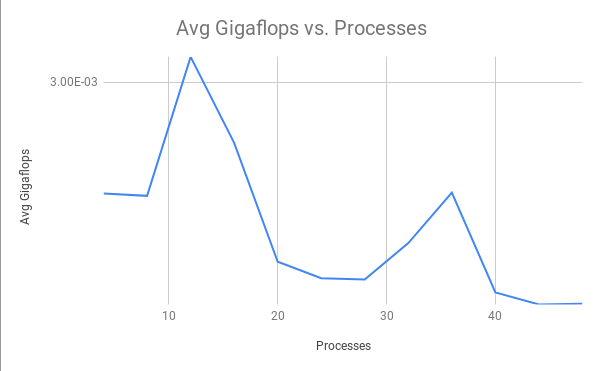
\includegraphics[width = \linewidth]{avgGig.png}
  \caption{Average $\frac{Gigaflop}{Second}$ vs. Number of Processes}
  \end{figure}
From the above graph it can be assumed that the workload was not siginificant to warrant an increase in overall performance. It appears that the overall performance is decreased the more the computation is distributed. I believe this is due to the fact that more processes corresponds to more time spent communicating between nodes. This leads me to believe a more complex workload will make the communication time less impactful to the overall performance results.

\clearpage
\end{document}
\begin{figure}
  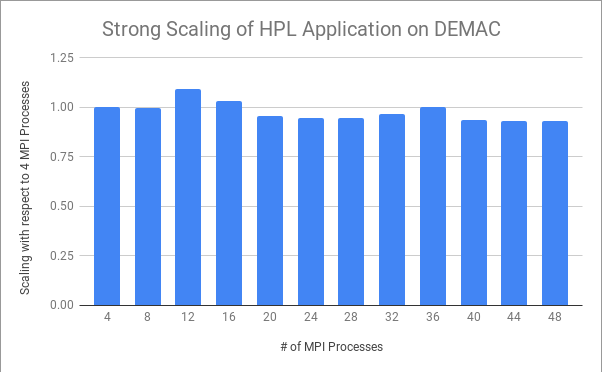
\includegraphics[width = \linewidth]{strongScaling.png}
  \caption{Strong Scaling}
\end{figure}

The above graph shows\ldots{}

\section{Auxillary Tasks}
In addition to working on the cluster, I have also completed a few tasks around the lab room including:
\begin{itemize}
\item Replacing the old printer
\item Sorting through, documenting, and removing duplicates from Dr. Gao's library
\item I'll fill this in later
\end{itemize}

\clearpage

\section{Future Work}
There is still much to be done in the future with the cluster specifically. The Parallella has both an dual-core ARM processor as well as the 16-core Epiphany coprocessor. As of now, MPI on the parallelas can only split computation between all the nodes using the two cores on the ARM processor on each node. This means that all of the power of the Epiphany coprocessor is not being utilized. To truly exploit the potential of this parallel cluster, I would like the opportunity to explore the Epiphany Software Development Kit (eSDK) that exposes the API for programming the epiphany chip, and see how it would be possible to combine MPI to use the full power of the Parallella boards and the DEMAC cluster. My goal for the end of Winter session is to successfully run a program with MPI that exploits the Epiphany chip.

In order to achieve this, I propose to start with an already existing MPI benchmark, profile to identify the hot regions of code that consume the most, and then create an implementation on the epiphany chip using the eSDK. This will allow me to explore scalability of an application across the cluster, and also get familiarized with the programming model on the parallella board.

\end{document}
\end{document}
